\section{Background and motivation}
\label{ch-introduction:sec:background}

Today's society and economy are highly dependent on the continuous availability of energy, or more specifically: electric energy.
In the UK, demand for electricity has increased over the past decades, and this trend is expected to continue into the future \cite{HMGovernment2009}.
This demand increase is only accelerated since a major focus of UK energy policies has been put on transitioning towards a low carbon economy \cite{RoyalAcademyofEngineering2010}.
Particularly the decarbonisation of heat and transport sectors are two areas of significant strategic focus and Low Carbon Technology (LCT) such as Photo-Voltaic (PV) installations, electric vehicles and heat pumps are expected to contribute significantly to this transition.

However, as adaptation of these LCTs increases and they start to penetrate power distribution networks, stress on these networks will continue to increase even further, which may result in additional service disruptions.
Furthermore, the uptake of LCTs is not expected to progress evenly throughout the entire power network, and instead clusters of early adopters are predicted to form, leading to certain Low-Voltage (LV) networks exceeding their operational constraints even at relatively low national rate of LCT adaption \cite{Poghosyan2014}.
The scale of this energy transition becomes becomes particularly apparent when referring to the UK's future energy scenarios that compare the predicted future load scenarios.

\begin{figure}\centering
	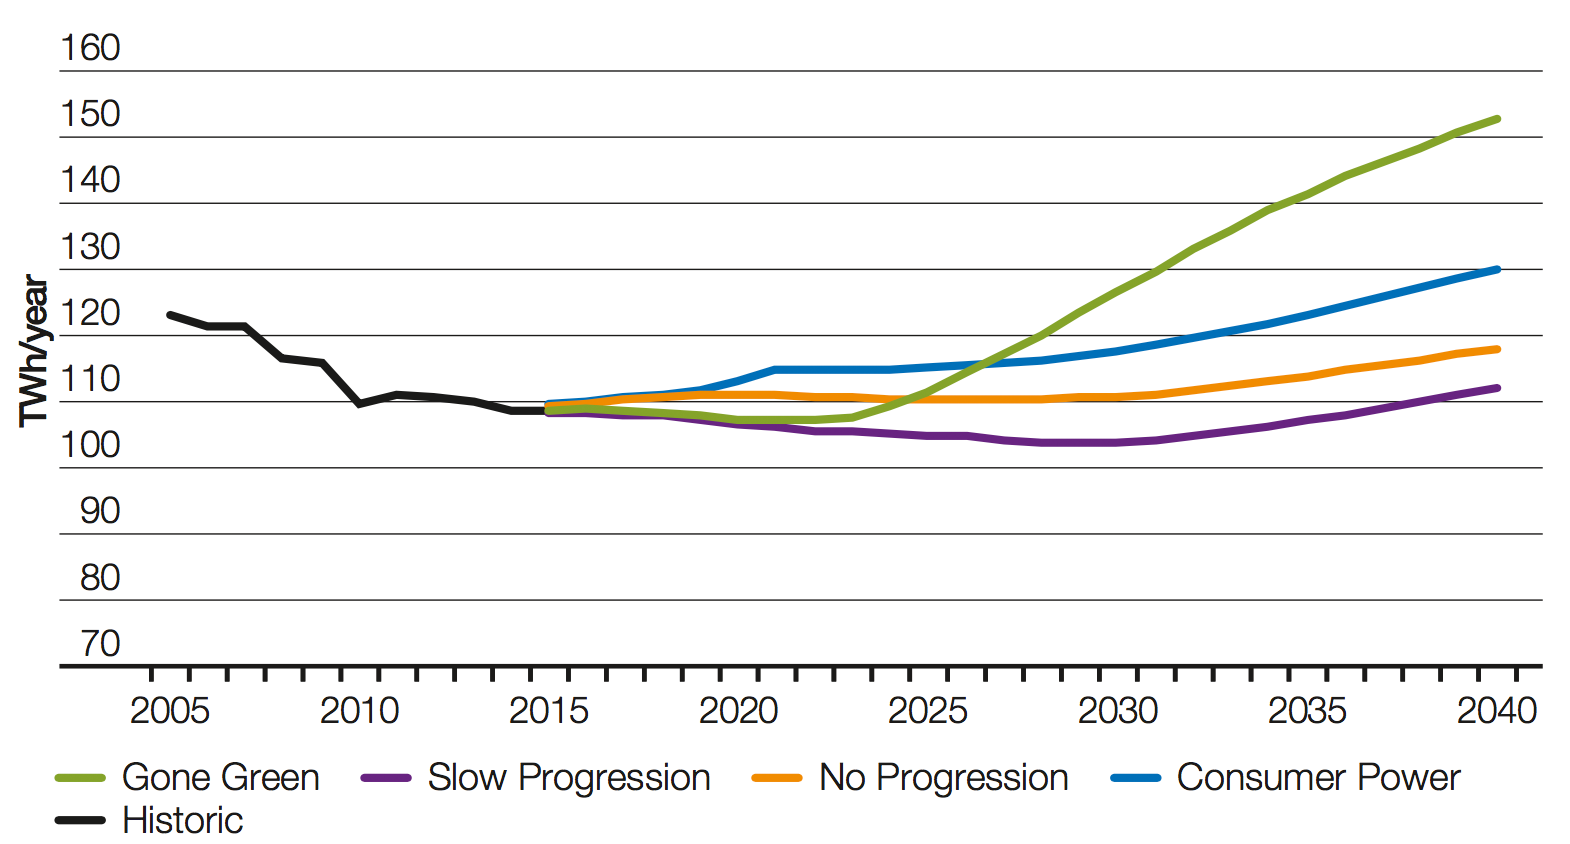
\includegraphics{_introduction/fig/electricity-demand-forecast}
	\caption{Annual residential demand for electricity from FES2016 \cite{FES2016}}
	\label{ch-introduction:fig:electricity-demand-forecast}
\end{figure}

Figure \ref{ch-introduction:fig:electricity-demand-forecast} shows the predicted increase in demand for electric energy when following the UK's 2020 and 2050 goals in reducing green-house emissions.
According to this projection, the annual energy demand will increase by more than 40TWh by the year 2040, if the ``Gone Green'' approach is implemented.
This trend is expected despite increasing device efficiencies, since the shift from oil and gas to electricity, i.e. the electrification, offset these gains.

\begin{figure}\centering
	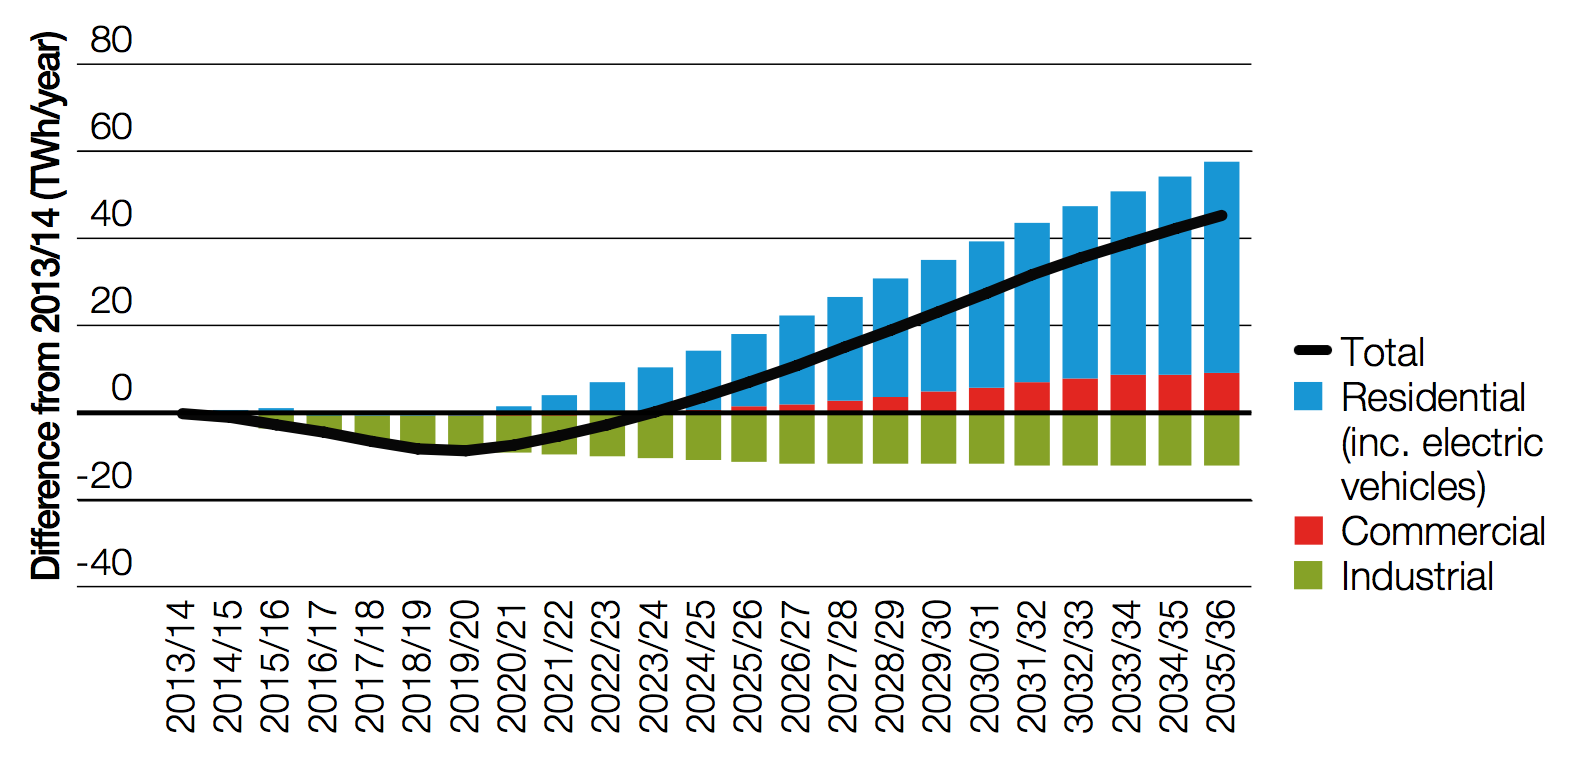
\includegraphics{_introduction/fig/electricity-demand-change-forecast}
	\caption{``Gone Green'' power demand comparison to 2013/14 by type (excluding losses) from FES2015 \cite{FES2015}}
	\label{ch-introduction:fig:electricity-demand-change-forecast}
\end{figure}

\nomenclature[G]{CREST}{Centre for Renewable Energy Systems Technology}

When breaking down the change in demand for electricity, as done in Figure \ref{ch-introduction:fig:electricity-demand-change-forecast}, one can observe how industry sectors are expected to decrease their energy consumption.
Yet residential and commercial sectors are expected to increase their demand and outweigh the industry's energy savings.
Their negative impact on the distribution network is only amplified, since loads in the residential and commercial sectors are typically situated at the network edge, i.e. in the LV distribution network.
This part of the network is its weakest part, since its assets were designed to caters for small powers between 315kVA to 500kVA \cite{EDS08-0115}.
A study based on the findings from \textit{Electricity North West} in \cite{ElectricityNorthWestLtd2014} emphasises the issues that result from residential increase in demand for electricity, of e.g. voltage deviation due to an uptake of LCTs.
As the number of PV installations is expected to grow, the voltage deviation magnitude and frequency is also going to increase \cite{Woyte2006}.
%The voltage deviation and corresponding power profiles are shown in Figure \ref{ch-introduction:fig:lct-impact}, which was produced by simulating several loads on the IEEE LV Test Case power distribution feeder.
%Loads were modelled at high resolution, using the \textit{Centre for Renewable Energy Systems Technology} (CREST) dwelling model \cite{Richardson2010a} and a subset of loads was adjusted using a normal and Rayleigh distribution for solar irradiance and home-charging EVs, respectively.
%The findings in Figure \ref{ch-introduction:fig:lct-impact} show how uncontrolled home-charging of EVs significantly reduces voltages in the network, and although solar injection does lead to voltage rises along the feeder, unbalanced injection increases voltage deviation even further.
%
%\begin{figure}\centering
	\subfloat[]{
		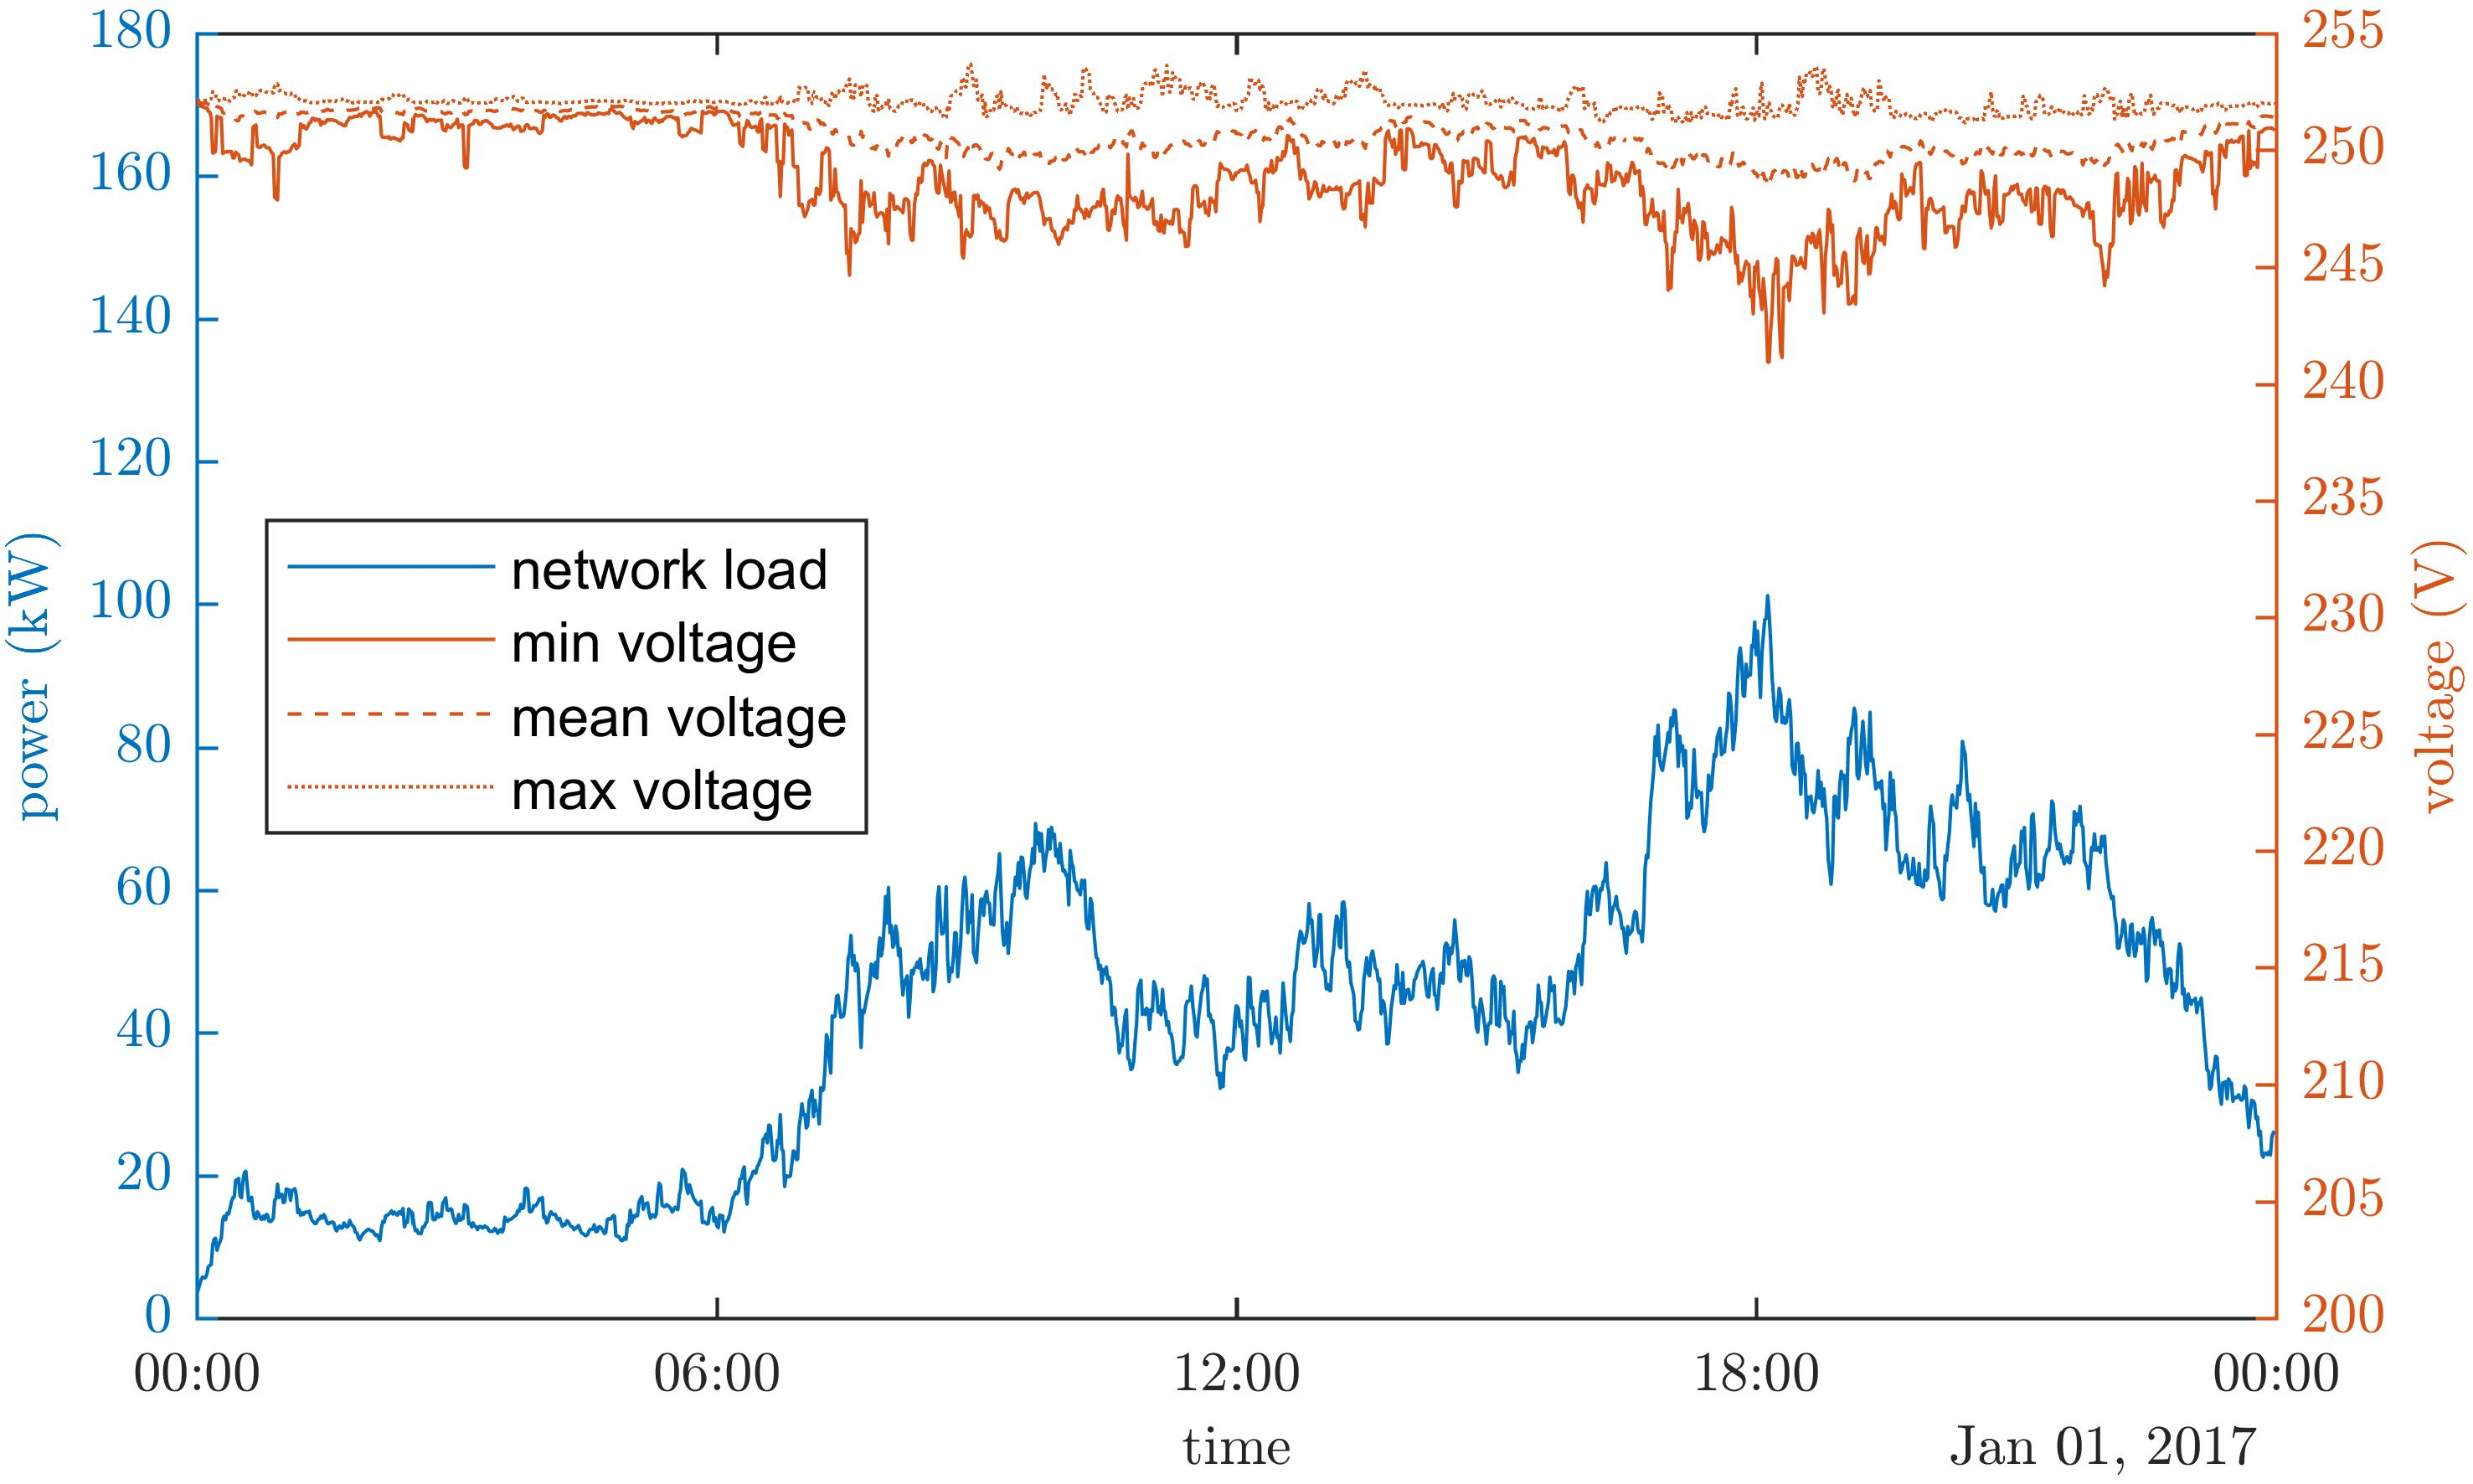
\includegraphics{_introduction/fig/lct-impact-without}
		\label{ch-introduction:subfig:lct-impact-without}
	}
	\vspace{1mm}
	\subfloat[]{
		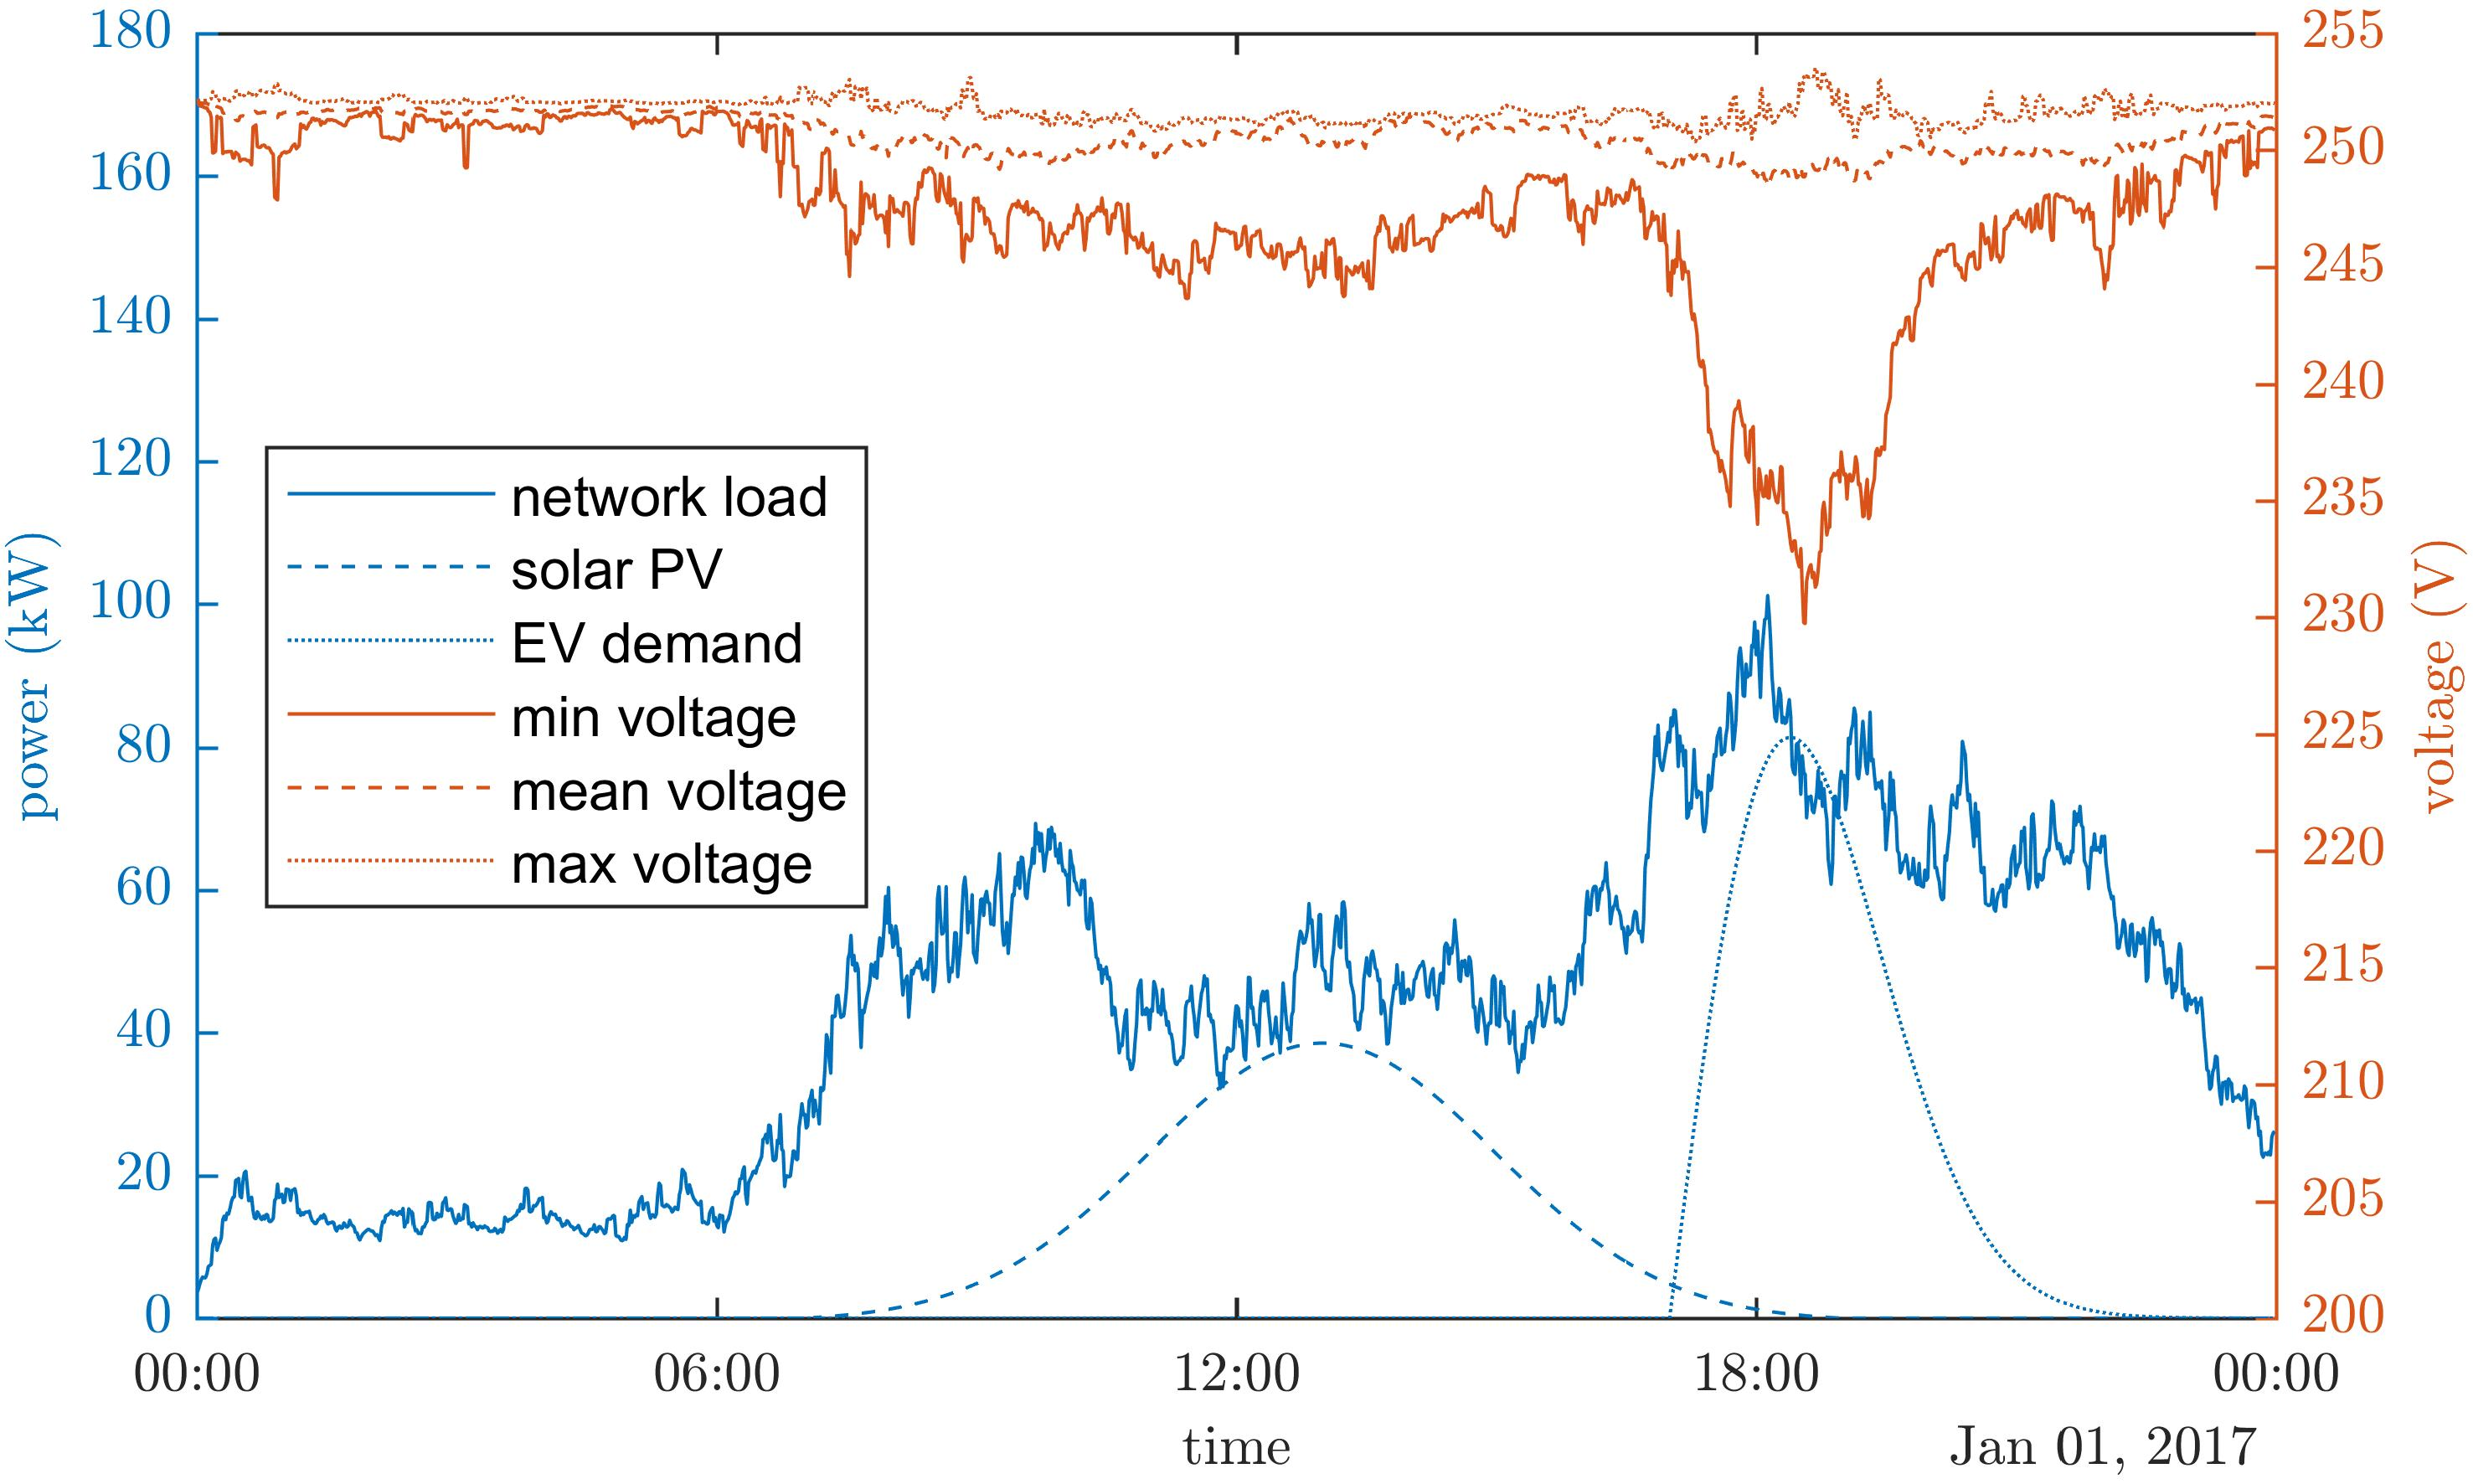
\includegraphics{_introduction/fig/lct-impact-with}
		\label{ch-introduction:subfig:lct-impact-with}
	}
	\caption{Study that compares impact on network voltages due to an uptake in LTCs on the IEEE LV test case: (a) does not contain any PV generation or EV loads; in (b) 20\% of all customers have PV generation with a peak generation of 3.5kW \cite{MongooseEnergy2015} and 20\% of all customers own EVs with Mode-2 home-charging capabilities at 7.4kW \cite{SustainableEnergyAuthorityofIreland2015}.}
	\label{ch-introduction:fig:lct-impact}
\end{figure}

Such a voltage drop behaviour was achieved with a relatively low rate of LCT adaptation in the residential environment, therefore strict regulation is in place to assure continuous operation without violating any operating constraints.
Otherwise additional voltage deviation, unbalanced network operation or potential asset overloads could be the result.

Traditional network planning approaches to follow these regulation were used to circumvent constraint violations.
These approaches follow the commonly used practice of aggregating a large number of customers and designing the power delivery network to cater for their largest probable demand, i.e. the After Diversity Maximum Demand (ADMD) method \cite{Richardson2010a}.
This ADMD method has remained the same for many years and uses historical load analysis and standard growth assumptions that are both no longer valid in this unprecedented LCT uptake scenario \cite{Yunusov2016}.
To make things worse, LV networks in the UK are generally unmonitored once installed.
Distribution Network Operators (DNOs) have become aware of this issue and are developing updated planning strategies involving ``smart'' and ``flexible'' electricity grids \cite{Fang2012}.
However, in situ equipment that will become subject to the same adaptation of LCT needs to be managed actively via innovation in the use of existing and new technologies; otherwise both frequency of service disruptions and customer minutes lost will increase alongside the proliferation of LCTs \cite{Ault2008a}.


\subsection{Topology and challenges of the UK low-voltage power distribution network}
\label{ch-introduction:subsec:topology-of-lv-network}

Today's UK electricity network has grown over the past century and is based on an interconnected high-voltage gird.
The largest part of this grid is also known as the transmission network, which connects centralised power stations to distribution networks.
Those distribution networks supply electricity to all loads across the mainland of the UK, including industrial, urban and rural customers\footnote[1]{Some small and remote UK islands like the Shetland islands are not connected to this national grid and have their separate electricity infrastructure. Therefore they are not considered as part of this thesis since the study of this kind of network lies outside the research scope.}.

The entire structure of the network is a three-phase Alternating Current (AC) system since this allowed easy voltage level conversion with the use of transformers, i.e. without the need of power electronics.
In the UK, the highest voltage level for generation and transmission is 400kV.
Such a high voltage requires a relatively small current to transmit the generated bulk power, which in turn reduces conduction losses and maximises the efficiency of the high-voltage network.
Regional supply points step-down this high voltage to 132kV\footnote[1]{In some cases regional supply points provide 127kV instead of 132kV.} to deliver power to Distribution Network Operators (DNOs).
From the primary level of the distribution network and onwards, this so called medium-voltage is stepped down to 33kV, then 11kV and finally 400V, in order to cater for heavy industry, medium clients and household sized customers, respectively.

\nomenclature[G]{DER}{Distributed Energy Resource}
\nomenclature[G]{ADMD}{After Diversity Maximum Demand}
\nomenclature[G]{OLTC}{On-Line Tap-Changer}

Primary substations in the UK are equipped with regulation equipment, e.g. On-Line Tap-Changers (OLTC), to increase or decrease the voltage on the secondary transformer side depending on the current level of demand.
Secondary transformers do not have such regulating equipment and instead apply a constant voltage conversion ratio which is set according to the network's typical demand.
This aim of this network regulation is to keep distribution level voltages within their statutory operating bands, i.e. 230V +10\% -6\% for the LV network as specified by the Electricity Supply Quality and Continuity Regulation (ESQRC) \cite{HealthandSafetyExecutive2002} and Engineering Recommendation G59 \cite{EnergyNetworksAssociation2013}.
In the UK, all households are connected to one of the three phases of the 230V distribution network.
To achieve a balanced network, each customer's phase allocation is chosen at random.
Also, throughout the majority of the power network's development period, customers were light consumptive loads, which meant that a reasonably predictable power flew from higher voltage levels towards the lower voltage levels.
Therefore, traditional network planning approaches to circumvent constraint violations, follow the commonly used practice of aggregating a large number of customers and designing the power delivery network to cater for their largest probable demand, i.e. the After Diversity Maximum Demand (ADMD) method \cite{Richardson2010a}.
However, this ADMD method has remained the same for many years and uses historical load analysis and standard growth assumptions, which are both no longer valid in this unprecedented LCT uptake scenario \cite{Yunusov2016}.

Firstly, because the injection of power from Distributed Energy Resources (DERs), e.g. rooftop solar PV, can reverse the power flow, and secondly, because large and volatile electrified products, e.g. home-charging Electric Vehicles (EVs), are predicted to significantly increase demand at peak times.
Such technologies have significant impact on the voltage stability \cite{Petinrin2016}, and combined with the expected increased in phase unbalance, traditional network management methods may no longer be able to effectively mitigate their negative impact.
This means that in situ equipment needs to be managed actively via innovation in the use of existing and new technologies; otherwise not only the frequency of constraint violations will increase, but also the frequency of service disruptions and customer minutes lost is expected to rise alongside the proliferation of LCTs \cite{Ault2008a}.
One such innovative technology, which is the main focus of the presented research, is the installation and management of battery storage \cite{Chen2009}, which is reviewed in the following section.


\subsection{Solutions to mitigate impact of LCT}
\label{ch-introduction:subsec:solutions-to-mitigate-impact-of-lct}

Two solutions exist, allowing DNOs to support LV network's operation: 
\begin{enumerate*}
	\item reinforcement of in situ network assets;
	\item deployment of network support equipment.
\end{enumerate*}
Whilst network reinforcement would certainly address immediate issues of current network capacity constraints, this approach is also the more expensive and disruptive option.
More specifically, customer will need to deal with outages during periods of asset upgrades (e.g. transformer upgrade and line re-conductoring after secondary transformers' tap settings have been adjusted).
Therefore, alternatives to defer or avoid network reinforcements have been sought and assessed \cite{Harrison2007, Zangs2016a, VanderKlauw2016d, Greenwood2017}.
Most promising alternatives are to install flexible and controllable Distributed Energy Resources (DERs), or more specifically: Battery Energy Storage Solutions (BESS) \cite{Wade2010}.
BESS has not only seen significant advancements in technology, but also received increasing attention in both academic studies and industry trials \cite{Palizban2016}.

Installing BESS on a strategic location in the LV network brings several advantages to DNOs' control over the network's performance.
Roles for BESS are addressed in the subsequent section, i.e. Section \ref{ch-literature:sec:role-of-energy-storage-a-survey}.
However, a few examples of potential benefits from BESS include the regulation of voltages to stay within statutory operating bands \cite{Yang2014}, shaving peak loads to relieve stress from the installed network assets \cite{Bennett2015}, and reducing phase unbalance to increase network efficiency \cite{Wang2015b} .
Whilst the questions regarding locating and scaling of BESS have mostly been addressed, BESS control can be split into two complementing yet unmarried approaches:

\begin{enumerate}
	\item ``off-line'' control, using load forecasts and BESS schedules \cite{Cecati2011, Chaouachi2013, Palma-Behnke2013, Khodaei2014}, and
	\item ``on-line'' control, using Set-Points Control (SPC), Model Predictive Control (MPC) or similar dynamic control methods \cite{Salinas2013, Huang2013, Huang2014a, Sun2014a}.
\end{enumerate}

Furthermore, with the anticipated uptake of household BESS, mechanisms to control several storage systems also need to be considered.
For instance, several industry leaders propose to store solar energy in order to support charging of EVs \cite{Baumann2017}.
Without rooftop PV installations, batteries need work in a cooperative manner to not impose additional strain onto the network.
The full review of storage control strategies to achieve both off-line and on-line, as well as centralised/individual and distributed battery control is presented in Section \ref{ch-literature:sec:control-of-energy-storage}.


\subsection{Smart control}
\label{ch-introduction:subsec:smart-control}

\nomenclature[G]{IoT}{Internet of Things}

As already mentioned in Section \ref{ch-introduction:subsec:solutions-to-mitigate-impact-of-lct}, off-line and on-line control strategies exist to manage BESS.
This traditional control often dealt with the dispatch of a single energy entity, but due to the distributed nature of the expected LCT uptake, methods to result in cooperative behaviour needed to be proposed.
With the penetration of smart meters and communication-enabled devices in the so called ``Internet of Things`` (IoT), power systems have the potential of becoming interlinked networks of smart devices, too.
So called ``smart control'' mechanisms complement the traditional off-line and on-line control strategies and are of great research interest to enable the uptake of distributed LCTs.

For example, ``smart charging'' is a key term that summarises EV charging mechanisms where the limited network capacity causes multiple EVs to share the available resource amongst themselves \cite{Sortomme2011, Vaya2012, Garcia-Villalobos2014}.
Intelligently limiting the EVs' maximum charging rates prevents them from adding unnecessary stress onto the network at the cost of longer charging times.
A similar key term is the so called ``smart grid'' where distributed resources communicate and cooperate in order to e.g. shed load using Demand Side Response (DSR) or maintain micrigrid operation in fault situations \cite{Samadi2012, Liu2014, Liang2014}.
The fundamental problem that is addressed in the research field of smart control is to find an optimal balance between network benefits and customer cost.
Also, the fundamental requirement for the successful realisation of smart control is the reliable exchange of information amongst the partaking smart entities.

Hence, smart control does not only require robust control mechanisms, but also a robust communications infrastructure.
Literature, which is reviewed in Chapter \ref{ch-literature}, shows that all control mechanisms dealing with the coordination of distributed energy resources either explicitly or implicitly assume a robust communication infrastructure.
For instance, this requirement is assumed when messages are received without delay and immediately after dispatched or when a single control instruction result in the synchronised reaction of all entities.
In reality however, the strength of the communication link may vary with e.g. weather or current network traffic, and fixed message delays and exact device synchronisation can no longer be guaranteed.
Therefore, not only smart control algorithms, but also their sensitivity to the strength of the underlying communications infrastructure is of interest.

\subsection{Challenges to control BESS}
\label{ch-introduction:subsec:motivation}

From the extensive catalogue of possible roles for energy storage in the electricity grid that was presented in Section \ref{ch-literature:sec:role-of-energy-storage-a-survey}, the focus of the research in this thesis is put on aiding DNOs to manage and operate their power distribution networks.
More specifically, battery energy storage is the main focus since is has the potential to defer or even mitigate costly network reinforcements.
Modern battery technology allows the storage of electrical energy in ever-decreasing form factory, whilst power electronics technology becomes more efficient at integrating batteries into power networks.

As shown in the literature review in Chapter \ref{ch-literature}, methods of controlling BESS to optimise power flow have been of great research interest.
However, the impact on particular key parameters of the three-phase networks still need to be investigated.
Subsequently, the challenge of applying real-time corrections to BESS schedules in order to decrease peak demand whilst obeying to technical and operational constraints is also a remaining research question.
Also, since the expected uptake of distributed LCTs through proliferation of household storage solutions (e.g. to counteract the impact of EVs) requires sophisticated coordination mechanisms, two additional research challenges have been identified.
The first challenge focuses on improving cooperating device behaviour despite communication disturbances (i.e. through message desynchronisation), and the second builds upon the findings from key network improvements to construct a functioning BESS control mechanism despite the absence of a telecommunications infrastructure.





